\documentclass[./\jobname.tex]{subfiles}
\begin{document}

\chapter{Task Description}

This project is about simulating and optimising a circulative traffic light control. The simulation is done with  \href{https://www.dlr.de/ts/en/desktopdefault.aspx/tabid-9883/16931_read-41000/}{SUMO} which stands for Simulation of Urban MObility. SUMO provides an API that allows external programs to cast and controll a simulation. These control structures, simulation evaluation as well as the optimisation algorithms are programmed in Python 3.7. \\~\\
The project includes the following tasks: 
\begin{itemize}
	\item create infrastructure to call simulation and alter simulation parametes in SUMO
	\item construct different intersections at different traffic loads
	\begin{itemize}
		\item Manhatten grid layout: 1x1, 1x3, 3x3
		\item traffic load: night, noon, rush-hour
	\end{itemize}
	\item four different optimisation algorithms
	\begin{itemize}
		\item NSGA2
		\item Conjugate Gradinet Descent
		\item Differential Evolution
		\item self created heuristic using Hill-Climbing
	\end{itemize}
	\item description and evaluation of the results
	\item precise technical report to ensure repeatability 
\end{itemize}

The simulation returns three parameters: 
\begin{itemize}
	\item overall waitingtime calculated as the sum of the waiting time of all cars
	\item overall number of stops calculated as the sum of the stops by all cars
	\item fairness in waitingtime calculated as the variance of the waitingtimes \\
\end{itemize}
We are looking for a solution that minimises all of these parameters. \\
All of the considered traffic load scenarios are stable. This means, that the waiting line does not grow arbitrarily larg. 

\newpage

\chapter{Simulation Infrastructur}
sumo environment, simulation runner, simulation parameter, reroute, tripinfofile and simulation result\\

\textbf{\underline{Problem:}} Since the cars can take a turn at every intersection, it might be possible that car gets trapped in the grid for a longer period. This aritficially increases the number of stopcounts and the waitingtime. The optimiser can not improve this situation because the traffic light has no impact on this issue. To prevent that this effect weakens the found solutions, the function evaluation must be adapted. This is done by normalising the waiting time as well as the stopcount with the length of the trip by that specific car. However this also implies, that the grid is equally spaced. 

\chapter{Algorithms}
This chapter describes the pseudocode and the characteristics of the implemented optimisation algorithms. Alltogether four different optimisers are compared: Differential Evolution (DE), Non Dominated Sorting Genetic Algorithm (NSGA II), Conjugate Gradinet Descent (CGD) and a self-created heuristic based on the Hill-Climbing (HC) principal. 

\section{Differential Evolution}

Differential Evolution was first published by \cite{storn_differential_1997}. New formes and adaptions are constently developed which belong to some of the best performing optimisation algorithms. The "framework" of Differential Evolution is described in \autoref{algo: DE}. 

\begin{algorithm}
	\SetAlgoNoLine
	\DontPrintSemicolon
	population $\gets$ initialization\;
	\While{g < $G_{max}$}{
		\For {individual $x_i$ \textbf{in} population} {
			$v_i$ = muation($x_i$, population, F)\;
			$u_i$ = crossover($x_i$, $v_i$, CR)\;
			\If {function($u_i$) < function($x_i$)} {
				$x_i$ = $u_i$\;
			}
		g = g + 1\;
		}
	}
	\unterschrift{Differential Evolution}{}{}
	\label{algo: DE}
\end{algorithm}

The framework allows different definitions of mutation and crossover. In this implementation the mutation $rand\textunderscore1$ is used. The following equation \ref{eq: mutation rand 1} describes this mutation operator. The subscript $i$ hereby stands for the current individual in the loop. The indizes $r1$ to $r3$ denote random but different individuals in the population. 

\begin{equation}
\label{eq: mutation rand 1}
v_i = x_{r1} + F (x_{r2} - x_{r3})
\end{equation}

The parameter $F$ is also called the scalefactor and can be choosen by the user. Typically this is set to be a number in the intervall $F = \left[ 0 ... 1 \right] $.

Further a binomial crossover strategy is used. For every coordinate $j$ in the vector, either an element of the old vector $x_i$ or a new vector $v_i$ is choosen. This again depends on a user defined parameter $CR$ called the crossover rate. To ensure, that at least on single element from the new vector is choosen, a random coordinate $K$ must be transfered. 

\begin{equation}
u_{ij}=\begin{cases}
v_{ij}, &\text{if $j = K \lor rand[0,1] \leq CR$}\\
x_{ij}, &\text{otherwise}
\end{cases}
\end{equation}

\section{Nondominated Sorting Genetic Algorithm II}
The NSGA-II was proposed by Kalyanmoy \cite{deb_fast_2002}. In contraty to the DE, this algorithms is able to optimise multiple functions at the same time. This is called a multicriteria optimiser. The result of this alogorithm are multiple individuals in a population. Ideally this population describes the pareto front. These are all feasible solutions, the user can then decide which optima is best suited. \\

The implementation was done in conjunction with the algorithm description in appendix \ref{chap: NSGA2_Description}. For a more convenient implementation and readability, every individual in the NSGA II is an object of the class individual which holds the most important attributes of a candidate. The following pseudocode \ref{algo: NSGA2} outlines the general steps to perform the NSGA II algorithm. 

\begin{algorithm}[H]
	\SetAlgoNoLine
	\DontPrintSemicolon
	population $\gets$ initialization\;
	\While{g < $G_{max}$}{
		\For {i \textbf{in} population/2} 
		{
			$p1$, $p2$ = tournament\textunderscore selection(Pt)\;
			$q1$, $q2$ = crossover($p1$, $p2$)\;
			$q1$ = mutation($q1$)\;
			$q2$ = mutation($q1$)\;
			Qt = Qt $\cap$ ($q1$, $q2$)\;
		}
		Rt = Rt $\cap$ (Qt)\;
		Rt = fast\textunderscore non\textunderscore dominated\textunderscore sort(Rt)\;
		Pt = crowding\textunderscore distance\textunderscore sorting(Rt, Pt.size)\;
		g = g + 1\;
	}
	\unterschrift{NSGA II}{}{}
	\label{algo: NSGA2}
\end{algorithm}



\section{Conjugate Gradient Descent}
Compared to the previous algorithms, the Conjugate Gradient Method is a deterministic algorithm which uses a numeric approximation of the gradient. This method is again capable of optimising scalar valued functions. \\
The original idea dates back to \cite{hestenes_methods_1952}. It is specially constructed for optimising quadratic problems of the form $f(x) = \frac{1}{2}x^T H x + b^T x$. If the problem can be represented in this form, the CGD takes exactly $n$ iteration where $n$ is the dimensionality of the function $f: \mathbb{R}^n \rightarrow \mathbb{R}$. \\
The following pseudocode \ref{algo: CGD} outlines the implemented steps of the CGD. This algorithm also holds two subfunctions: \textit{numGrad} calculates the numeric gradient with the central differencing scheme and the \textit{linsearch} implements a golden section search starting from point $x$ and along a vector $d$. 

\begin{algorithm}
	\SetAlgoNoLine
	\DontPrintSemicolon
	$x$, $d$ $\gets$ initialization\;
	\While{$||\nabla f(x) || < \epsilon$ OR $||\hat{\eta}\textbf{d}|| < \epsilon$}
	{
		grad = numGrad(x)\;
		$\textbf{d}$ = $-grad$ + $\frac{||grad||^2}{||grad_{old}||^2 \textbf{d}}$\;
		\If {$\frac{grad\text{ }\textbf{d} }{||grad|| \text{ }||\textbf{d}||}$ > $-\alpha$} 
		{
			$\textbf{d}$ = -grad\;
		}
		$\hat{\eta}$ = linesearch(f(x, $\textbf{d}$))\;
		$x_{old}$ = x\;
		$grad_{old} = grad$\;
		$x = x + \hat{\eta} \textbf{d}$\;
	}
	\unterschrift{Conjugate Gradient Method}{}{}
	\label{algo: CGD}
\end{algorithm}


\section{Hill Climbing}

The Hill Climbing methode is a very simple from of optimisation algorithm. This method again optimises scalar valued problems. The general idea is to sample points around the current location, and select the new location based on the fitness values of these points. There are two main concepts, that need to be figured out to make the process work are: 
\begin{itemize}
	\item generating new solutions 
	\item step-size adaption\\
\end{itemize}

In this implementation, new solutions are produced by going a step in positive and the negative direction of each coordinate. If two consecutive steps do not result in a better solution, the step-size is adapted by halven it. The main issue with this method is, that it performs a strong local search and ultimately leads to a premature convergence. \\

The following pseudocode \ref{algo: HC} describes the necessary steps. 

\begin{algorithm}[H]
	\SetAlgoNoLine
	\DontPrintSemicolon
	$x_start$ $\gets$ initialization\;
	\While{fe < $\#FE_{max}$}{
		\For {d \textbf{in} Dim} 
		{
			z[d] = step\;
			$y_{1,2}$ = $x$ $\pm$ $step$\;
			f = funcion(y)\;
			fe = fe + 1\;
		}
		\If {function($y_d$) < function(x)} 
		{
			$x$ = $y_d$\;
		}
		\Else 
		{
			$step = 0.5 * step$ 
		}
		
	}
	\unterschrift{Hill Climbing}{}{}
	\label{algo: HC}
\end{algorithm}


\chapter{Scenarios}
sumo cross, reroute probability (Abbiegewahrscheinlichekit), LP, qin max

\chapter{Experiments}

\section{Preparation}

\subsection{calculations relative green}

The following image \ref{fig:greenphases} shows the green phases for each intersection.

\begin{figure}[H]
	\centering
	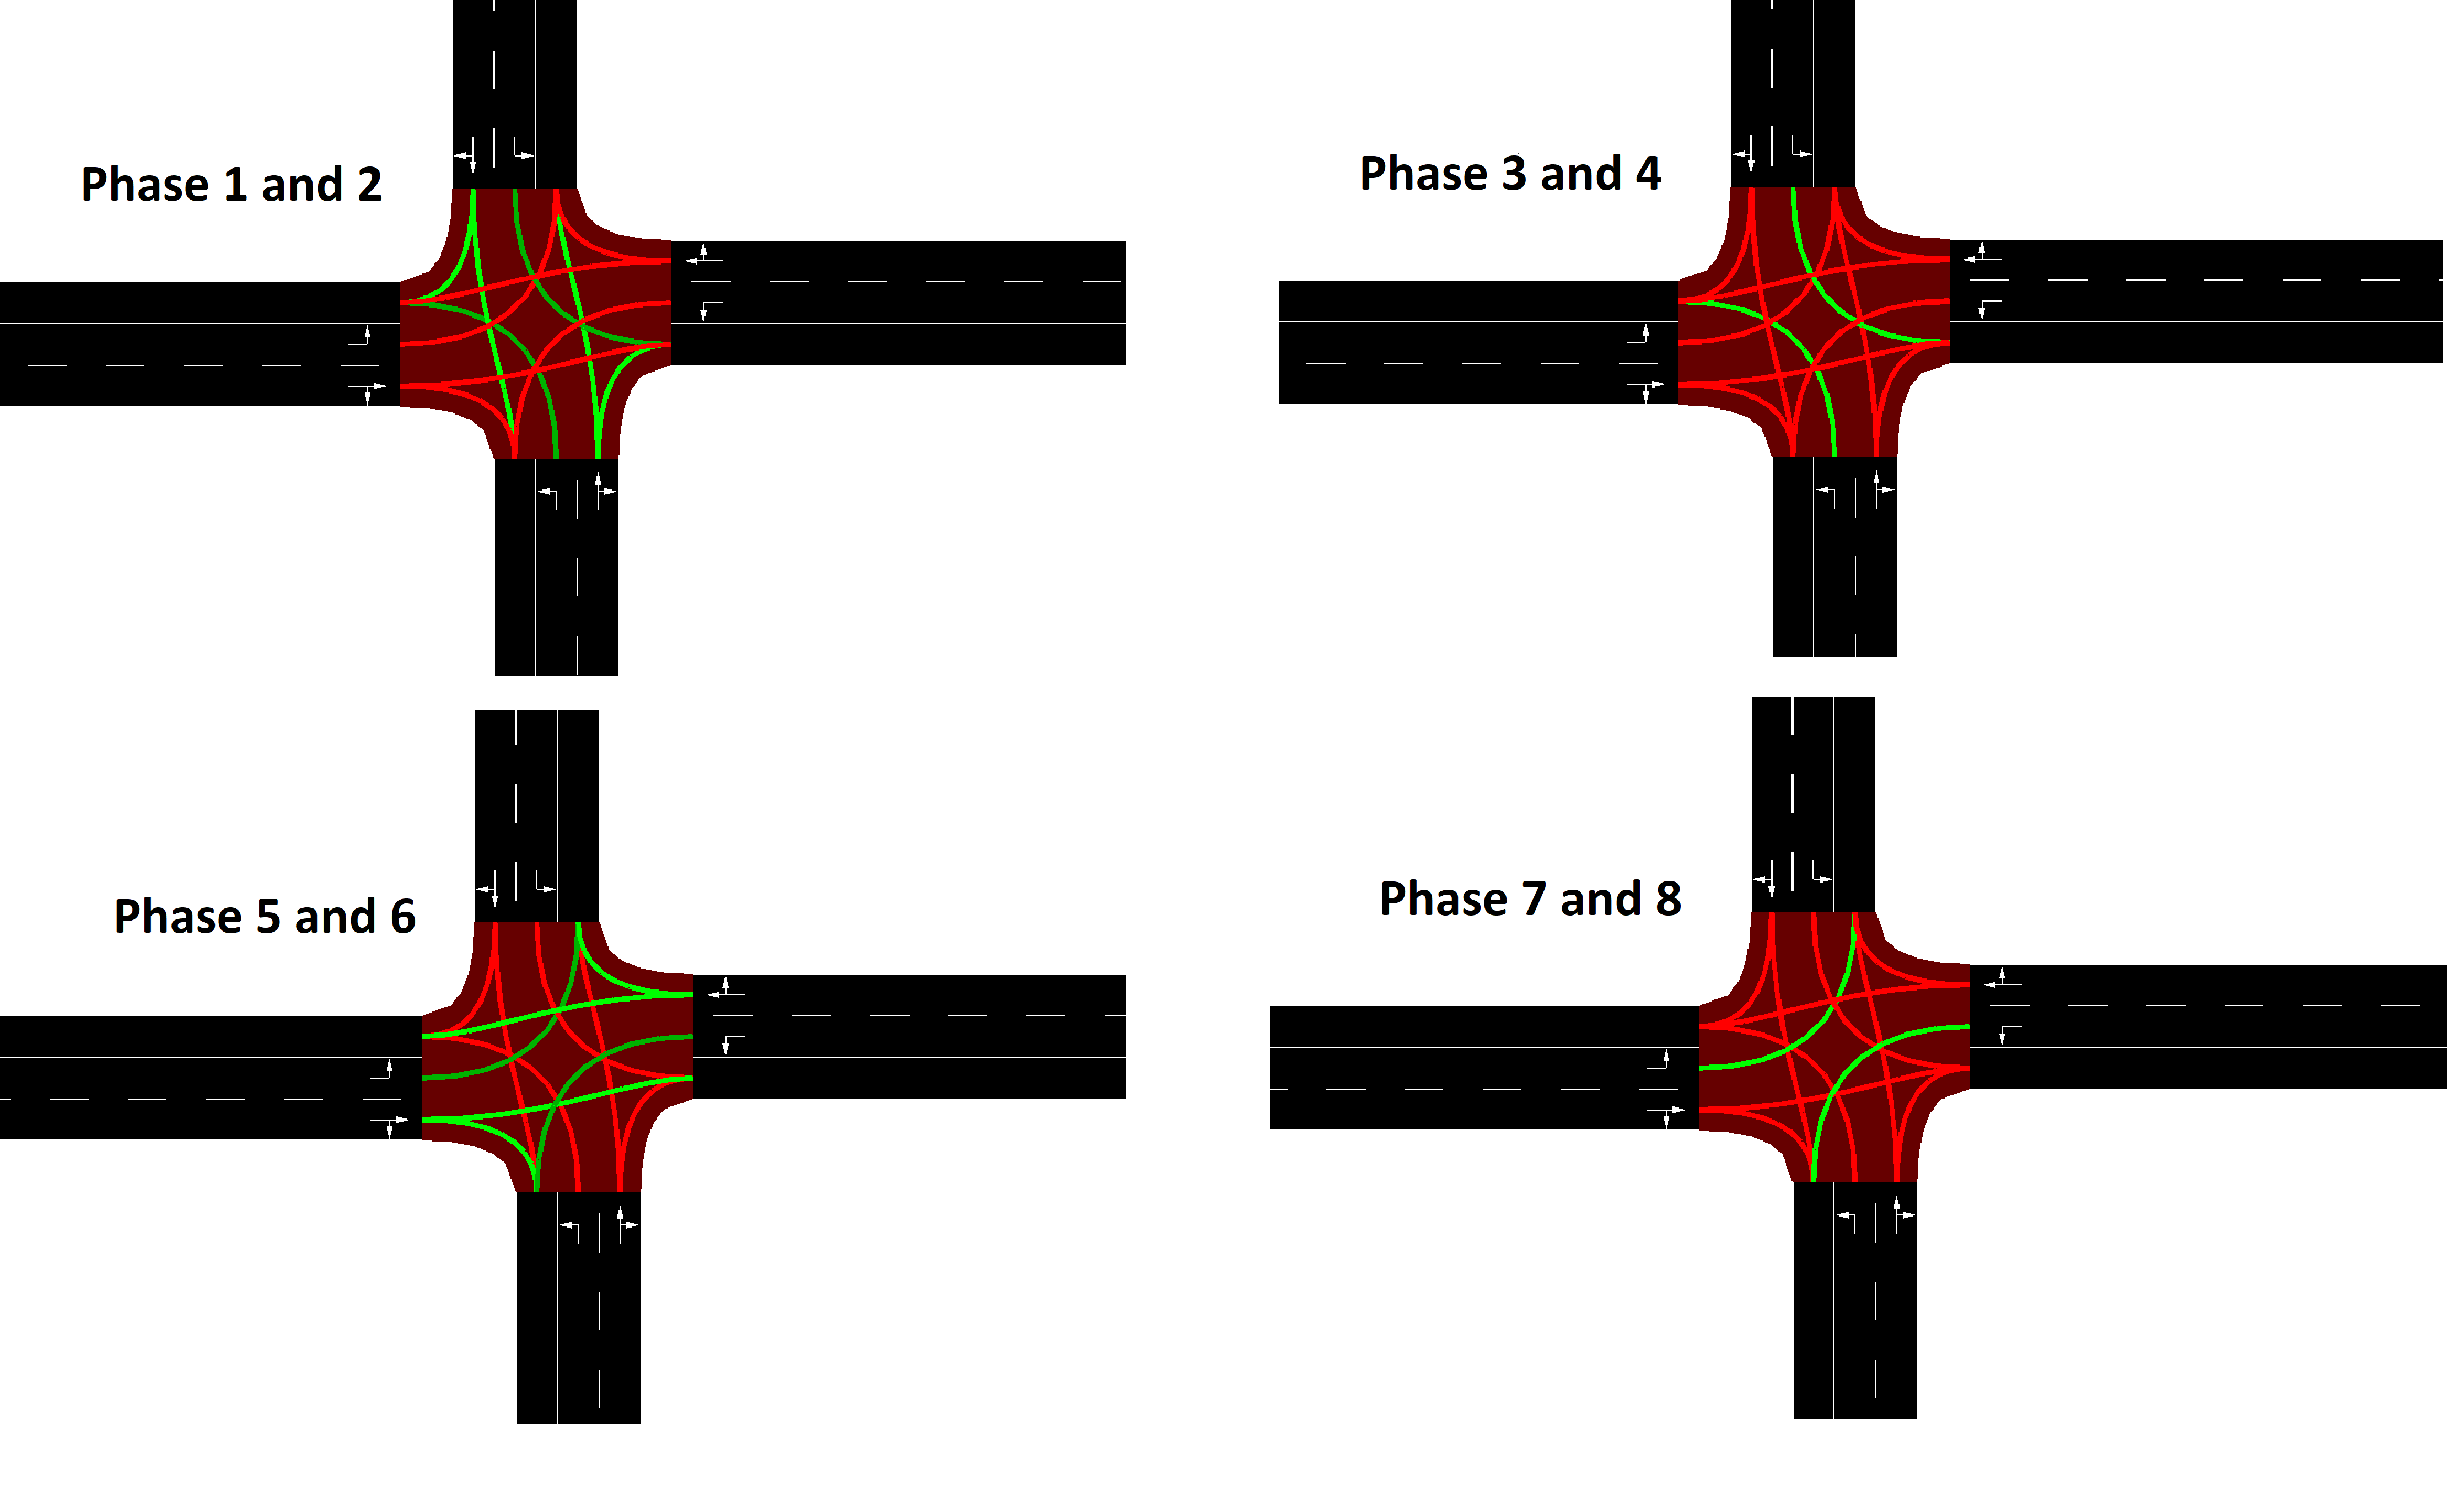
\includegraphics[width=1\linewidth]{../img/png/cross_phases.png}
	\unterschrift{traffic light phases for each intersection}{}{}
	\label{fig:greenphases}
\end{figure}

The calculation of the relative greens phases is related to the input stream into the intersection. If we call the input stream from the street i $I_{i}$ and the turn probability from the i-th street to the j-th street $p_{ij}$, then we can determine the relative green time using an weighted average. Note that the streets are numerated from 1 (north) increasing clockwise to 4 (west). For the first relative green time (seen in figure \ref{fig:greenphases}, upper left corner) we get the following calculation:

\begin{equation}\label{key}
rg_{phase 1} = \frac{max(I_{1}(p_{13} + p_{14})+I_{3}(p_{31}+p_{32}))}{\sum_{i=1}^{4}phase_{i}} 
\end{equation}

This is because, we have an input stream from street 1 divided (according to the turn probabilities) into street 3 ($I_{1}p_{13}$) and street 4 ($I_{1}p_{14}$). The same is done for the input stream $I_{3}$. Then this value is divided by the sum of all green phases. This procedure is then used to calculate all four phases.

\section{Results}

\chapter{Conclusion}

\end{document}
